\chapter{Часть 1}

Эта история - о людях, которых Родина отправила защищать небо чужой страны. О лётчиках, бывших частью грандиозной мощи военно-воздушных сил красной сверхдержавы - и об их визави, чью страну с трудом можно найти на карте. О людях, знавших, что вслед за ними придут тысячи. И о людях, знавших, что кроме них - некому.

Эта история о битве Давида и Голиафа. В которой Давид не мог победить - слишком неравны были стороны - но смог доказать гиганту, что есть что-то ещё кроме грубой силы, и заставил считаться с собой.

Эта история о командировке советских лётчиков в Египет - и о том самом знаменитом бою с израильтянами над Сохненской долиной 30 июля 1970 года. Или “Римон-20” - как называют его в Израиле.

…
\begin{textcitation}
	$\ldots$
	теперь снимаются все запреты и ограничения на пилотаж и боевое маневрирование. Воздушную подготовку мы должны начать с чистого листа и руководствоваться в ней своим здравым смыслом, а не чужой совестью,
\end{textcitation}
--- такими словами напутствовал своих летчиков заместитель главного советника по авиации в Египте, генерал-лейтенант Дольников в начале августа 1970-го года.

За этими словами скрывалось внезапно пришедшее осознание того, что советские лётчики неожиданно для них попали на на очередные учения, а на настоящую войну, где мишень летит непредсказуемо и имеет наглость стрелять в ответ, и стрелять боевыми. Где нет ограничений безопасности, потому что воевать вообще небезопасно. Где инстинкты важнее учебников. Где можно по-настоящему быть сбитым - и быть убитым тоже по-настоящему. А ещё за этим скрывалось осознание того, что противник просто оказался сильнее и хитрее. Об этой истории в советских ВВС вообще не любили говорить - разве что тихо, полушепотом. События одного дня той египетской командировки двух советских эскадрилий наложили огромный отпечаток на всю дальнейшую подготовку лётчиков, для нескольких из которых их египетское путешествие разделилось на “до” и “после” - а для некоторых “после” не было вовсе.

В этой и последующих статьях мы поговорим о том, как и почему это произошло. И могло ли всё сложиться иначе.

Несколько слов об использованных источниках:

В качестве основного источника для этой статьи использовались в первую очередь воспоминания людей, непосредственно участвовавших в защите неба Египта (или их израильских оппонентов). В нескольких случаях, использованы воспоминания их сослуживцев, не участвовавших в той командировке, а также советских военнослужащих тех времен, не бывших в Египте, но имевших достаточно информации о произошедшем. В случае, если описанное в воспоминаниях участников противоречит друг другу, об этом будет явно написано. Полный список источников будет приведен в конце 3-й части.

\section{Я русский советник}

Эта история берет начало 6 июня 1967 года, когда на Ближнем Востоке началась очередная война. Шестидневная. Арабы снова собирались сбросить евреев в море, и советский генштаб был абсолютно уверен в их, арабов, победе. Но израильтяне имели свой взгляд на будущее страны.

\begin{figure}[h!tb] 
	\centering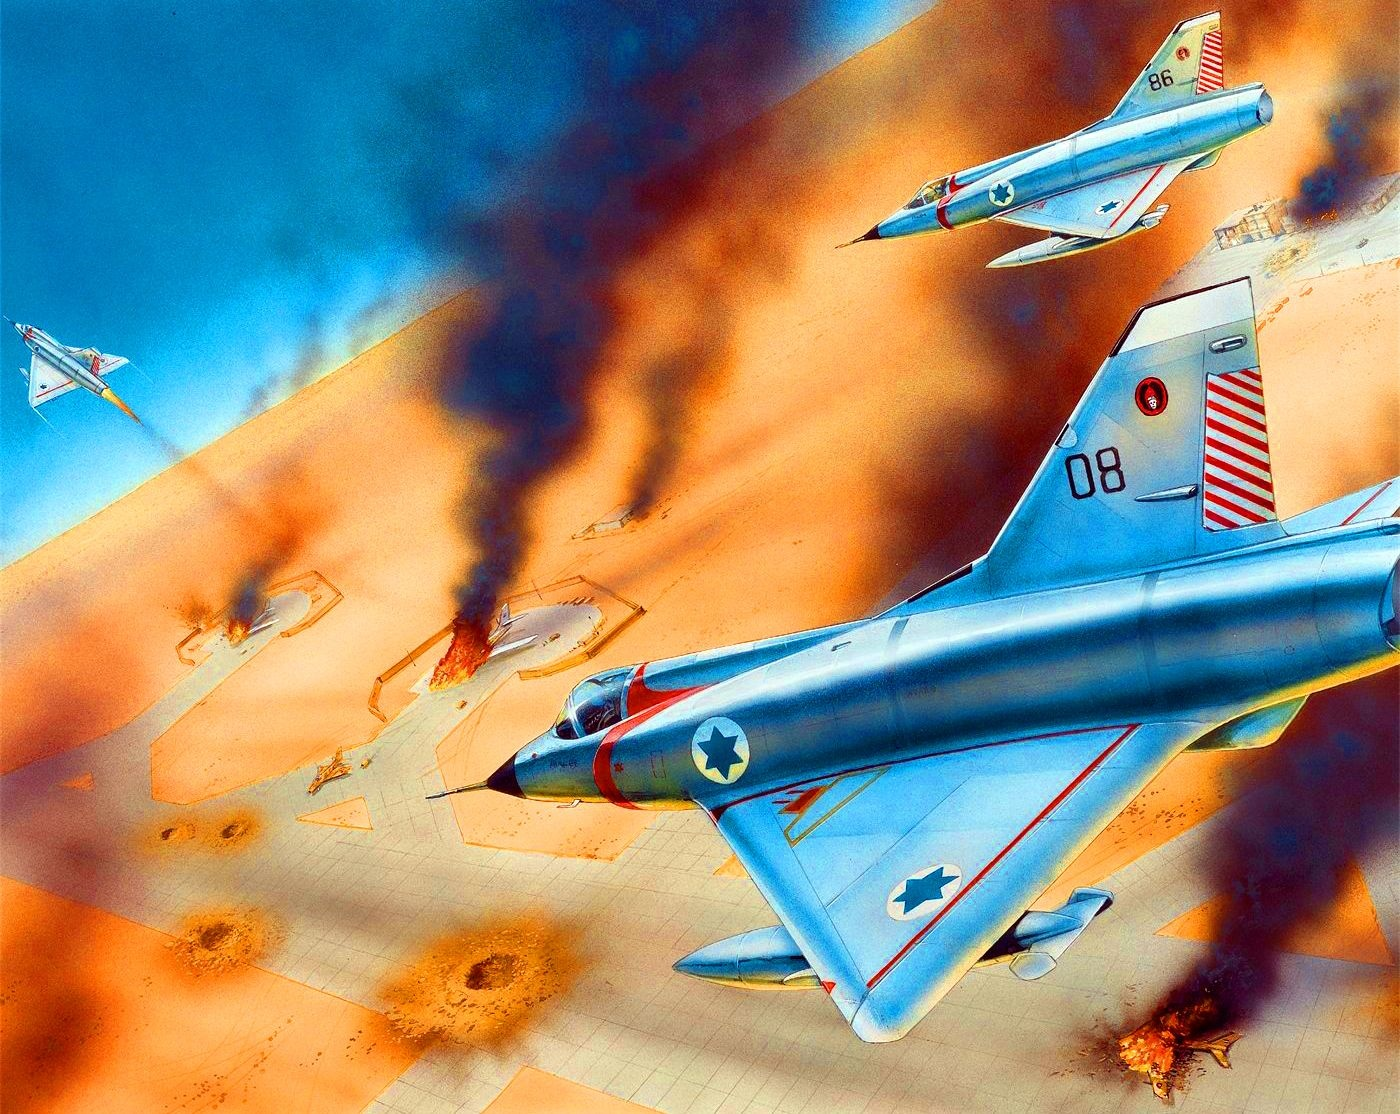
\includegraphics[scale=0.4]{Dolina_1/3bsutm8WQ9I.jpg}
	%	\label{fig:scipion} % Unique label used for referencing the figure in-text\end{document}
	%	%\addcontentsline{toc}{figure}{Figure \ref{fig:placeholder}} % Uncomment to add the figure to the table of contents%----------------------------------------------------------------------------------------
	\caption{Пара «Миражей» 101-й эскадрильи атакует египетский аэродром}%	CHAPTER 2
\end{figure}

рабская коалиция обладала колоссальным превосходством: в числе, в самолётах - особенно самых современных, МиГ-21. Израиль не мог противопоставить им такое же число машин - а потому пошел другим путем. Рано утром 6 июня 1967 года арабская авиация была уничтожена совершенно внезапным, гениальным, потрясающе отрепетированным ударом с воздуха. Особенно пострадали египтяне - от их ВВС практически ничего не осталось. Разгром был полный: израильская авиация непрерывно бомбила бегущие египетские войска на Синае, сирийские - на Голанах, иорданские - на Западном берегу - и им нечего было противопоставить. Небом завладели серебристые самолёты с бело-синей звездой Давида.

Шесть дней унижения прошли - война закончилась. Для Египта встал вопрос, что делать дальше? Единственный возможный ответ был для египтян прост и очевиден: обратиться за помощью к своему “Большому брату”, СССР, с просьбой прислать новое оружие взамен бездарно потерянного во время бегства с Синая. Союз не отказал - правда теперь вместе с техникой там высадился большой десант военных советников, которые должны были сделать так, чтобы египтяне наконец перестали позорить советскую технику.

Арабские ВВС того времени представляли собой эклектичный набор разных самолётов - английских, советских, чешских; их (ВВС) структура часто была малопонятна даже для самих летчиков. К тому же после синайской катастрофы 67-го года египтяне напрочь провалили мораль и лишились веры в собственные силы. Что хуже, они лишились почти всех самолетов, огромного количества танков (из трофеев в Израиле потом создадут 2 танковых бригады), грузовиков, оружия…

С началом лавины новых советских поставок вопрос с матчастью более-менее решился. Тут же встал ничуть не менее сложный: как научить египтян воевать так, чтобы вся эта техника снова не досталась Израилю? Для этой цели и прибыла новая группа советников. Советовали они на уровне дивизий, бригад, полков, в генштабе и на аэродромах - советские военные специалисты проникли в египетскую армию глубочайшим образом, чтобы научить тех, кого можно научить и перестроить то, что должно быть перестроено. Что делать с теми, кого научить ничему нельзя — не уточнялось.

Предполагалось, что они будут давать рекомендации с высоты собственного опыта - на самом деле, им пришлось практически заново учить египтян воевать. Полковым советникам - с нуля вбивать в головы офицеров самые простые вещи, начиная с азов. Советникам в генштабе - реформировать структуру армии, что сложнее, пытаться донести какие-то вещи до египетских генералов... Дело было не простым и требовало значительного терпения. И времени.

Чуть легче, чем всем остальным, приходилось советникам в ВВС. Египетские ВВС - это вообще вещь в себе, своего рода военная аристократия со всеми соответствующими атрибутами настоящей аристократии: чувством собственной исключительности и убежденности в собственном величии. И серебряной ложкой, конечно. Но даже там принятые порядки иногда шокировали - например, телесные наказания провинившихся, совершенно невозможные в реальности советского человека. Всё-таки этот советский человек, выросший в культуре определенного “равенства”, был по духу гораздо ближе к израильтянам, чем к арабам.

Сами египетские лётчики в большинстве своём обладали двумя чисто арабскими качествами - болезненным самомнением и помноженным на него нежеланием совершенствоваться. Разумеется, были исключения в виде десятков талантливых пилотов. Проблема заключалась в том, что сама египетская армия всячески сопротивлялась возможным изменениям и буквально исторгала из себя слишком умных “выскочек”. Проявление излишней инициативы в ВВС Египта было весьма нежелательным: чересчур инициативный пилот мог быть слишком “вольнодумным” и политически нелояльным. А лояльность в арабском мире ценилась куда выше, чем профессионализм. И правда, что могло пойти не так?

В начале 1969 года египтяне активизировали удары по израильским войскам на Синае - началась “война на истощение”. Египет имел колоссальное преимущество в «стволах» артиллерии в районе канала, примерно в 8-10 крат. Понятно, что вести артиллерийские дуэли при таком соотношении сил израильтяне не могли, а потому они традиционно отвечали ударами с воздуха. Там картина принимала совершенно привычный оборот - в боях “пара на пару” и “звено на звено” серебристые “Миражи” в большинстве случаев легко одерживали верх. Египтяне теряли самолёты, пилотов и остатки веры в себя. Советники недоумевали. Египтяне злились: “Не так, не правильно нас учите!” Советники отвечали: “Наши тактики и наши самолёты - лучшие в мире! Это вы - плохие, негодные ученики…”

Иногда это противостояние — египтянина и советника — принимало трагические формы - так, один из командиров 104-й истребительной авиабригады как-то заявил своему советнику, что тот больше ничему не может его научить и предложил убраться из его эскадрильи куда-подальше. А в ответ на возражения - предложил разобраться по-мужски, в воздухе - кто лучший пилот. В результате “дуэли” египтянин не справился с самолетом на сверхмалой высоте и разбился, а советник был немедленно отправлен на Родину.

Этот случай был далеко не единственным (правда, произошел он уже после окончания войны на истощение), он стал известен лишь благодаря своему трагическому исходу. Негласное противостояние “египетский офицер - его советник” было практически на всех уровнях. Опять же, советские лётчики - люди весьма гордые и самоуверенные, много чего видевшие, и арабские порядки часто вызывали у них брезгливость. К тому же, в Египте были лучшие из лучших, первоклассные пилоты. Правда, в настоящих воздушных боях они никогда не участвовали, но были совершенно уверены, что евреи - это как американцы, и при необходимости с ними вполне можно воевать. И побеждать - как американцев во Вьетнаме. А все проблемы арабов, они от арабской лени и безалаберности, а не от того, что они ежедневно сталкивались с противником, о возможностях которого советские офицеры не имели практически никакого представления. С израильскими летчиками.

Египтяне безнадежно проигрывали. После того как в конце 1969 в Израиле появились американские “Фантомы”, длинная рука Хель ХаАвир смогла дотянуться до любой точки Египта, перенеся войну с района Суэцкого канала в египетский тыл. Египтяне не были готовы к тому, что под ударом окажется вся территория их страны — они то начинали войну только в районе Канала, надеясь, что этой территорией бои и ограничатся. К концу 1969 года всё шло к тому, что Египет проигрывал войну, которую сам развязал.

\section{Президент Насер и его кошмары}

В начале декабря 1969 Насер приехал в Москву. Тайно (об этом визите не было написано ни строчки в прессе), без протокольных мероприятий, без огласки. Его положение было критическим - Хель ХаАвир господствовали в воздухе, где развернулась самая настоящая охота на египетские истребители и батареи ПВО.
Насер приезжает даже не требовать и не просить - практически умолять Брежнева спасти его от евреев.

Он просит не только новое оружие и советников - он просит отправить советских солдат. То есть - о прямом военном вмешательстве СССР. Сначала ему закономерно отказывают - впрочем, у египетского лидера есть отличный аргумент. “Если сейчас Египет проиграет - кто знает, кто после этого окажется у власти? И кого из сверхдержав этот кто-то выберет своим главным союзником? Если русских смущает то, что Египет не входит в Организацию Варшавского Договора - так Египет готов вступить туда хоть завтра!” Аргументы Насера оказываются убедительными, и вскоре министру обороны СССР Андрею Гречко на стол ложится план секретной операции “Кавказ”. Он предусматривал размещение на территории Египта крупной группировки регулярных советских войск, которые способны противостоять ВВС Израиля и которые выстроят непробиваемый ракетный щит на пути израильских самолётов и надежно прикроют египетские тылы от рейдов «Фантомов».

Фактически, Советский Союз вступал в очередную арабо-израильскую войну на стороне арабов. В качестве воюющей стороны.

\begin{figure}[h!tb] 
	\centering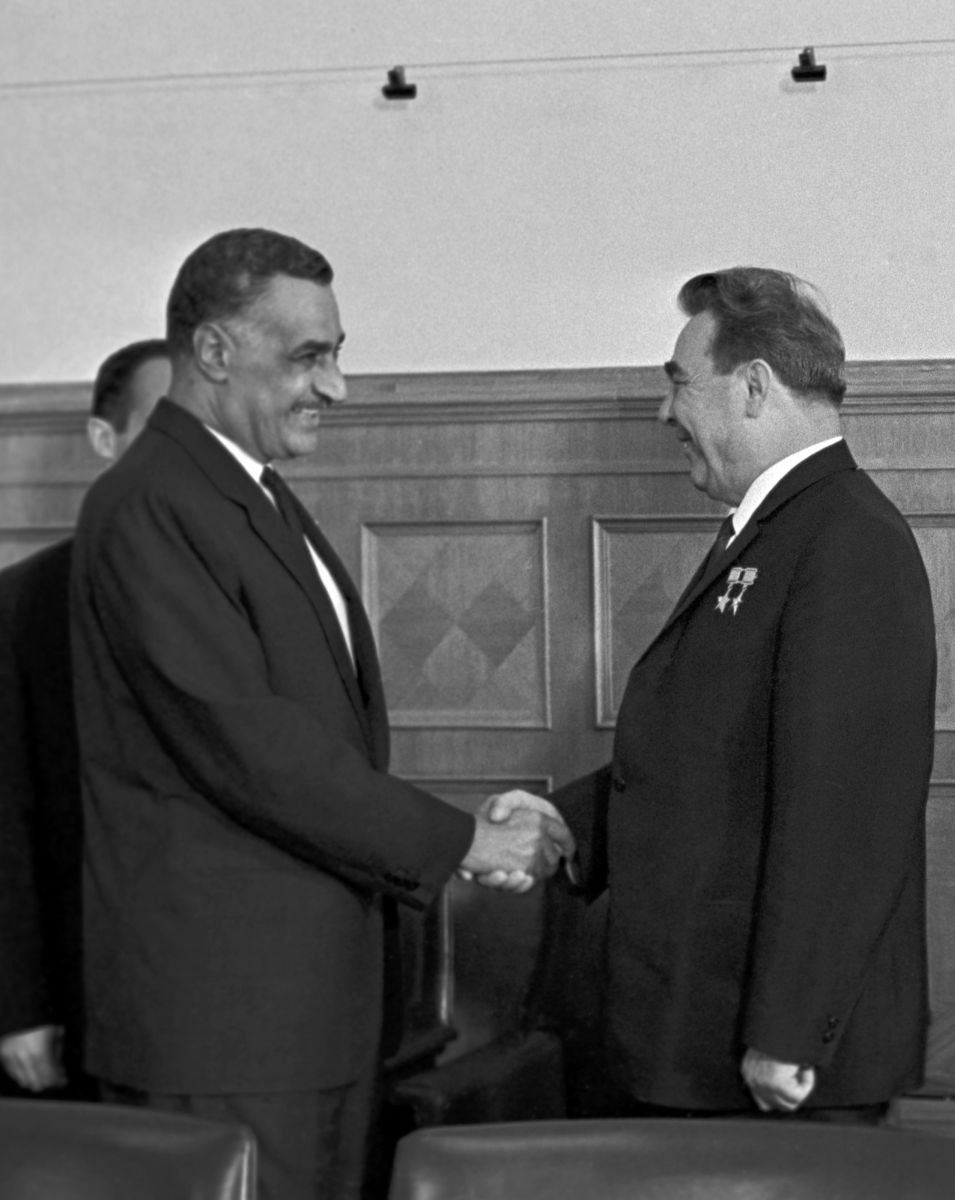
\includegraphics[scale=0.4]{Dolina_1/Zbp75LzED2Y.jpg}
	%	\label{fig:scipion} % Unique label used for referencing the figure in-text\end{document}
	%	%\addcontentsline{toc}{figure}{Figure \ref{fig:placeholder}} % Uncomment to add the figure to the table of contents%----------------------------------------------------------------------------------------
	\caption{Насер и Брежнев}%	CHAPTER 2
\end{figure}

Насер хотел, чтобы СССР открыто выступил на его стороне. В крайнем случае, он предлагал всех советских военнослужащих объявить добровольцами. Брежнев тогда ответил: “Нам никто не поверит, что нашлось воевать в чужой стране столько добровольцев. И вообще – мы так не привыкли”. Действительно, СССР, в отличие от американцев, предпочитал действовать тихо, без лишнего шума и огласки, желательно — под видом местных. Именно так решено было действовать и на этот раз. В СССР всерьез верили, что можно тихо и бесшумно перебросить в Египет несколько тысяч человек под носом у американцев и израильтян. Очень скоро грядущая операция стала секретом Полишинеля - и израильтяне, и американцы объявили о ней ещё до того, как первый советский корабль пришвартовался в Александрии, и это тоже выглядело весьма комично.

В общем, страхи египтян можно было понять. Самолёты со звездой Давида на крыльях стали для них настоящим кошмаром. С сентября (когда в войну вступили американские “Фантомы”) по декабрь 1969 они сумели сбить всего один “Мираж” и один “Скайхок”, потеряв 15-17 машин в воздушных боях, и ещё около 10 - от действий израильского ПВО. “Фантомы” и “Скайхоки” буквально выкашивали египетские зенитно-ракетные дивизионы, а “Миражи” охотились на “МиГи” над их собственными аэродромами. 9 сентября израильтяне провели знаменитый “Равив” - рейд вдоль Суэцкого залива на трофейной бронетехнике. Эффект был потрясающий: колонна из 6 трофейных Т-55 и нескольких БТР под командованием Баруха Хареля, сопровождаемая “Скайхоками”, прокатилась по египетским позициям, в буквальном смысле раздавив несколько РЛС, постов береговой обороны и одного египетского генерала, который принял колонну “Тиранов” за египетские танки и попытался остановить их - напрасно. Потери израильтян составили 3 человека и один “Скайхок” (его пилот, бывший старший замкомэска 102-й эскадрильи, а на момент гибели «пилот по необходимости» Хагай Ронэн, погиб).

Что важнее для нас, 9 сентября погибли двое военных советников в египетских частях ПВО - полковник Корнеев и майор Карасев. Что стало причиной их гибели: столкновение с танкистами Хареля, удары ВВС или что-то ещё - не известно.

На следующий день после окончания рейда у президента Египта Насера случился сердечный приступ. Ещё через день египтяне решили ответить массированным ударом с воздуха: МиГ-17 и Су-7 под прикрытием МиГ-21 должны были атаковать позиции израильской армии на Синае. И если первая волна бомбардировщиков более-менее успешно сумела выйти на цели и благополучно вернуться за Канал, то вторую и третью с распростертыми объятиями встретили две эскадрильи “Миражей”. Результат был удручающим: израильтяне заявили 11 сбитых самолётов (Египет признает потерю 8) при собственных потерях в 1 “Мираж” (в воздушном бою, летчик - первый израильский ас, капитан Гиора Ромм попал в плен). Египтяне претендуют на три сбитых “Миража” - правда, пилотов всех трёх почему-то зовут Гиора Ромм, при это один Гиора Ромм погиб, а два других Гиоры попали в плен. В декабре 1969 Ромма и комэска 102-й эскадрильи“Скайхоков” Ниссима Ашкенази, сбитого в августе, обменяли на 75 египтян, в том числе двух летчиков.

Стало понятно, что несмотря на все усилия, Египет проигрывает. И дело идёт к нокауту, а не поражению по очкам. Вот потому Насер отправился к единственному человеку, который мог его спасти. И вот почему тот не отказал.

В декабре 1969 в соответствии с решением Политбюро министр обороны СССР Маршал Советского Союза Андрей Антонович Гречко подписал приказ о создании на территории Египта системы ПВО, состоящей из регулярных советских частей.

Одних советников оказалось недостаточно. Голиаф отправился на войну лично — операция “Кавказ” началась. 

\section{Советские лётчики, египетские самолёты}

Вопреки устоявшемуся мнению, решение об отправке авиагруппы (в составе истребительного авиаполка и отдельной разведывательной эскадрилье) в братский Египет было принято задолго до знаменитого декабрьского визита Насера, в августе 1969. Командир 35-й отдельной разведывательной авиационной эскадрильи Юрий Настенко вспоминал об этом так:

\begin{textcitation}
	В пятницу, 1 августа 1969 года, после ночных полётов я возвратился домой. Вся семья сидела у стола: такой был обычай. Раздался звонок телефона дальней связи, который в столь неурочный час означал нечто непредвиденное. Меня вызывали в штаб воздушной армии. В пути я мучительно размышлял, зачем вызывают к командующему.
	Так и не придя ни к какому выводу, я переступил порог кабинета командующего воздушной армией генерал-лейтенанта авиации Василия Самсоновича Логинова. Военный совет был уже в сборе. Доложив о прибытии, я получил приглашение сесть.
	От сердца отлегло: ничего страшного не случилось. Тогда зачем вызов? Первый вопрос, который задали мне, содержал и ответ. Знаю ли я, что происходит на Ближнем Востоке. Я понял: еду на Ближний Восток.
	Следующий вопрос, который Василий Самсонович задал мне, был предельно ясным. Как я отношусь к предложению возглавить группу добровольцев-пилотов для оказания интернациональной помощи египетскому народу в отражении израильской агрессии. Двадцать лет меня готовили для того, чтобы ответить на этот вопрос утвердительно. Другого я не мог себе и представить. Так мы были воспитаны и воспитаны правильно.
	На следующий день специальным самолётом я вместе с другим таким же командиром полка, полковником Константином Андреевичем Коротюком (затем он стал генерал-майором), летел на беседу к министру обороны Маршалу Советского Союза А.А. Гречко.
	Из той встречи мне запомнился весьма примечательный момент. Когда один из моих лётчиков (на встрече присутствовали от каждого полка по одному командиру звена) на вопрос министра обороны начал громко произносить заученные лозунги о том, что мы самые сильные и умелые и победа будет за нами, начальник Генерального штаба Маршал Советского Союза М.В. Захаров, который, казалось, до этого дремал, поднял глаза и, обращаясь ко мне и полковнику Коротюку, сказал: «Разгромите ли вы супостата, не знаю, но вы должны Родине и семьям вернуть пилотов живыми, а не привезти их в цинковом гробу». И добавил: «Хвастунов с собой не брать, они первыми бегут с поля боя».
\end{textcitation}

Забегая вперёд, Настенко с этой задачей справился.

\begin{figure}[h!tb] 
	\centering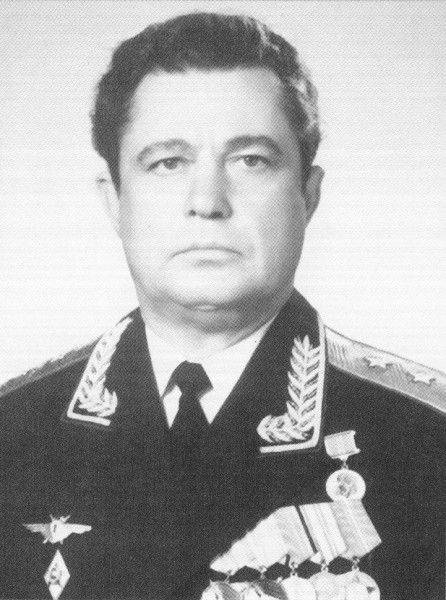
\includegraphics[scale=0.4]{Dolina_1/a9-qXqEZvKU.jpg}
	%	\label{fig:scipion} % Unique label used for referencing the figure in-text\end{document}
	%	%\addcontentsline{toc}{figure}{Figure \ref{fig:placeholder}} % Uncomment to add the figure to the table of contents%----------------------------------------------------------------------------------------
	\caption{Полковник Юрий Васильевич Настенко (впоследствии генерал-лейтенант ВВС)}%	CHAPTER 2
\end{figure}

Для отправки в Египет в Союзе была сформирована авиационная группа в составе двух авиабригад (по египетской терминологии), состоящая из отдельной эскадрильи (30 самолетов, 42 летчика) и одного полка (60 летчиков и 40 самолетов).

35-я разведывательная эскадрилья была укомплектована только советскими военнослужащими - и лётчики, и технический состав эскадрильи прибыли из СССР. В 135-м авиаполку ситуация была несколько иной: там из СССР прибыли только офицеры-лётчики и техники, остальную часть личного состава составляли арабы. В большинстве своём они прошли обучение в СССР, говорили по-русски и были в целом лучше подготовлены, чем персонал египетских частей.

“Разведывательной” она была только формально - её основной задачей были не полёты над Синаем, а защита египетского неба.

Снова вспоминает командир 35-й эскадрильи Юрий Настенко:

\begin{textcitation}
	На подготовку летного состава мне был дан один месяц. Всех летчиков я знал по фамилиям и именам, так как три года проходил службу в одном из полков 283 истребительной дивизии, из которой формировалась эскадрилья. Но тридцать суток — срок короткий. Летали каждый день, перелетая с одного аэродрома на другой, с берегов Черного и Каспийского морей, иногда по два раза в день. Об уровне подготовки летного состава можно судить по тому, что на воздушные стрельбы по летающим мишеням эскадрилья прилетела и произвела посадку в наихудших погодных условиях. Находившийся на этом аэродроме командир корпуса пво заметил по этому поводу, обращаясь ко мне: «Да, с этими пилотами воевать можно». Да, летать и стрелять мы умели, а воевать — нет. В течение дня и ночи ракетами и огнем из пушек было сбито 12 мишеней, причем все с первой атаки. Подготовка была закончена.
\end{textcitation}

В.Б.Ельчанинов в книге "Дан приказ ему…в Египет!" так описывал подготовку к советских лётчиков к командировке:

\begin{textcitation}
	Последние месяцы уходящего 1969 года в авиационных городках были наполнены динамичной боевой учебой. Личному составу истребительного авиационного полка было чем гордиться. На полигоне в ходе учений летчики, офицеры боевого управления, инженеры и техники добились отличного результата. Например, в течение одного дня в качестве целей было запущено 5 радиоуправляемых мишеней в стратосфере и 8 фронтовых крылатых ракет (для безопасности - без боевого заряда).
\end{textcitation}

Летчики уничтожили все цели при минимальном расходе ракет. Высотные цели были уничтожены всего шестью ракетами. Более сложной задачей было уничтожение фронтовых крылатых ракет, летящих на малой высоте и на скорости 900–1000 км/час. Солнце основательно разогрело пустыню и стало сложно выделить сигнал головки ракеты с тепловой системой наведения, а кучевые облака, имеющие высокую отражающую поверхность, становятся настоящими тепловыми ловушками. Несмотря на эти обстоятельства, все восемь целей не долетели до цели, были сбиты двадцатью ракетами.”

В общем, в течение месяца советские лётчики и техники занимались интенсивной подготовкой в Марах. К чему они готовились? К маневренным воздушным боям? Не совсем. Они готовились перехватывать цели по команде и наведению с земли - приблизиться, отстреляться. Но что будет, если цель вдруг начнет маневрировать?..

Фактически, отрабатываемые на полигонах перед отправкой в Египет навыки советским лётчикам просто-напросто не пригодились. Было бы любопытно узнать - в СССР вообще хоть как-то пытались анализировать действия израильской авиации? Судя по тому, что пишут участники тех событий, таких попыток практически не было. Иначе “фирменные” приемы израильтян - дежурство на малых высотах, демонстративные группы - не стали бы для них сюрпризом.

О составе израильских ВВС советские летчики тоже получили минимум информации. По воспоминаниям одного из них, основным противником считалась 101-я эскадрилья - якобы сборное соединение из лучших пилотов Израиля (на самом деле — обычная строевая эскадрилья, одна из трех в ВВС). Шла психологическая накачка летчиков — наши самолёты лучшие, наши тактики лучшие, враг будет разбит, победа будет за нами. То есть это, конечно, занятие нужное и важное — но не в ущерб реальным знаниям о противнике. Серьёзно, в какой-то момент советским лётчикам рассказывали, что на стороне Израиля воюют американские пилоты. Это отличный пропагандистский ход — проблема в том, что к реальности это не имело никакого отношения. Да, в Хель ХаАвир были люди, родившиеся в США - но репатриировавшиеся задолго до попадания в ВВС. Зачем доносить до своих пилотов заведомую ложь — мне не понятно.

В общем, наши пилоты просто были не готовы ко встрече с израильтянами. Что ещё хуже — в Каире советские командиры были просто не готовы управлять этими самыми пилотами, управлять боем. Проблема была даже не в том, что средний израильский пилот (а средних в том известном бою не было — были самые лучшие) был сильнее среднего советского. Проблема была в том, что условный Моти Ход по уровню понимания воздушного боя превосходил условного Григория Дольникова на голову. На порядок. На целую пропасть.

Вместе с лётчиками в Египет отправились и самолёты. Принято считать, что это были новейшие (производившиеся с 1969 года) МиГ-21МФ - экспортная, но практически неотличимая от “оригинала” модификация МиГ-21СМ. По сравнению с теми модификациями МиГ-21, которые были у египтян, этот самолёт был существенно более совершенным: новый двигатель Р13-300 был мощнее своего предшественника почти на 15\%, вследствие чего самолёт быстрее разгонялся и набирал высоту. В отличие от египетских самолётов, имел он и БРЛС (Сапфир-21), правда её ценность в условиях Ближнего Востока несколько снижалась - превосходная видимость позволяла значительно раньше, чем в Европе, увидеть противника глазами.

Вооружение советских машин тоже было существенно лучше - помимо 4 ракет Р-3 (АА-2 “Атолл”), МИГ21-МФ наконец имел серьёзное пушечное вооружение - сдвоенную ГШ-23 с полноценным боезапасом в 100 снарядов на ствол (против НР-30 с 60 снарядами у египетских МиГ-21 Ф-13 и вообще отсутствующей пушки у египетских МиГ-21 ПМФ).

Пожалуй, только в одном новые советские "МиГи" уступали предшественникам - из-за появления встроенной пушки советским конструкторами пришлось пойти на сокращение запаса топлива. Из-за установки более мощного двигателя на всех режимах вырос расход топлива. В результате эффективная дальность самолёта, и без того не блестящая, ещё сократилась. Фактически, советский лётчик при прочих равных условиях был вынужден раньше покидать бой - что, как выяснилось, имело все шансы стать для него фатальным. Но об этом мы ещё поговорим.

С самолётами, правда, есть одно противоречие - часто пишут, что они были получены “из состава” авиации ВМФ (черноморского флота), что в случае с модификацией МФ - экспортной - было весьма затруднительно. Кроме того, есть известное фото лётной книжки Владимира Михайловича Рожкина, лётчика, находившегося в Египте в с конце 1970 по середину 1971 года, где указано, что он летал на модификациях М и УС. Последняя нас мало интересует - это учебная спарка. Кроме этого, на ряде фотографий советских самолётов достаточно хорошо видно наличие только двух (а не четырёх, как на МФ) пилонов для ракет “воздух-воздух”.

Всё это наводит на мысли о том, что самолёты, попавшие в Египет в составе двух советских эскадрилий, были разных типов - часть была новой (МФ), часть - получена из состава авиации черноморского флота (вероятно, 562-го одесского авиаремонтного завода). Это не является критически значимым моментом, но добавляет некоторые штрихи к картине.

\section{Люди с той стороны Канала}

Когда советские лётчики готовились к выполнению интернационального долга где-то в небе над Крымом, их будущие оппоненты тоже тренировались. Правда, тренировки у них были несколько другого рода. Как и мишени, которые вовсе не хотели быть мишенями, и каждый раз старались ужалить в ответ. Да и цена ошибки, цена поражения была совсем другой - запредельной. Все прекрасно знали, что случалось со сбитыми лётчиками-евреями, когда (и если) они попадали в плен.

Однако же самые жаркие, самые яростные воздушные бои на Ближнем Востоке происходили отнюдь не над Египтом. Арабы в большинстве своём были слабым противником - но у израильтян всегда была возможность сразиться с равными себе. Собственной тенью. Собственными товарищами. И к учебным боям с ними относились - как к настоящим. “Ограничения безопасности? Зачем их придумали?! Там, за Каналом - они помогут уйти от ракеты? Там, в небе, есть только я и мой самолёт! - и такой же парень, изо всех сил старающийся вырваться из паутины прицела. И не важно, что на земле он вновь станет лучшим другом, сейчас - сбить, сбить его, мерзавца! Из последних сил. Открывая новые грани возможностей самолёта. И - себя. Не получается? Импровизируй! Лети на грани сваливания, рискуя врезаться в “противника”, на любых перегрузках. Всё ради одной цели - сбить его!»

Советские пилоты были бы счастливы иметь такие же возможности, как их израильские коллеги. Вот только вместо этого они имели тонну инструкций и встроенного в эскадрилью замполита - такого же лётчика. И когда бело-синяя сборная училась воевать, красная - училась четко исполнять инструкции. Возможно, это было разумно в большой войне с американцами. Но в войне с евреями это было фатальным.

В замечательной книге о пилотах 201-й эскадрильи “Фантомов” ВВС Израиля “От имени неба”, Авирам Баркаи дал великолепное описание тому настрою, который был совершенно типичен для всех израильских пилотов, не только “Фантомов”:

\begin{textcitation}
	Они были напористы до наглости, полны веселья и жизнерадостны, решительны и грозны, как ковбои. Они чувствовали себя другими. И были такими. Заточенная эскадрилья. До сумасшествия. Всё на границе возможного. Этих ребят нужно было силой удерживать в рамках. Всё, что у них было в голове - это воздушные бои. Отстаньте с бомбардировками, дайте сбивать. В программе полётов написано, что надо произвести тренировки бомбометания. Ну и что, что написано! Быстренько выполнили, что написано, и перешли на главное дело. Воздушные бои в разных условиях. Превысили ограничения G? Обнулили датчик. Раз, два, потянули! «Нагнали» 5G, чтобы не поймали, что надули. Инструкция гласит, что на посадку надо заходить на 19 градусах атаки со скоростью 150-160 узлов, и тогда самолёт приземляется как по маслу. Не в эскадрилье 201 – здесь никто не садится на 19 градусах. Низкий заход на посадку, прыжок над ЛЭП высокого напряжения в Кфар Ахим, приземление в середине ВПП, тормоза до упора, рывок рукоятки тормозного парашюта и молитва, чтобы не оторвался… Психопаты!
\end{textcitation}

В те времена в лётной школе ВВС Израиля для каждого курсанта существовал только один итоговый критерий успешного окончания лётного курса. Инструктора школы, они же - действующие боевые лётчики, собирались вместе и задавали друг другу один простой вопрос - готов ли я воевать вместе с этим парнем? Готов ли я доверить ему свою жизнь?

И про всех людей, оказавшихся в кабине самолёта с той стороне Канала, однажды кто-то сказал: “Да, я готов воевать вместе с ним”.
